% Graphic for TeX using PGF
% Title: /home/satenske/cours/AP/obj3/uml2.dia
% Creator: Dia v0.97.1
% CreationDate: Thu Sep 22 09:54:15 2011
% For: satenske
% \usepackage{tikz}
% The following commands are not supported in PSTricks at present
% We define them conditionally, so when they are implemented,
% this pgf file will use them.
\ifx\du\undefined
  \newlength{\du}
\fi
\setlength{\du}{15\unitlength}
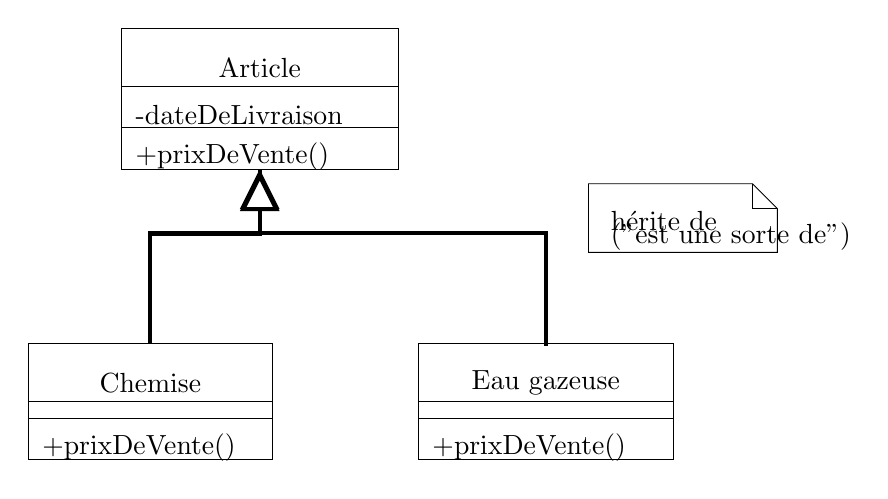
\begin{tikzpicture}
\pgftransformxscale{1.000000}
\pgftransformyscale{-1.000000}
\definecolor{dialinecolor}{rgb}{0.000000, 0.000000, 0.000000}
\pgfsetstrokecolor{dialinecolor}
\definecolor{dialinecolor}{rgb}{1.000000, 1.000000, 1.000000}
\pgfsetfillcolor{dialinecolor}
\pgfsetlinewidth{0.020000\du}
\pgfsetdash{}{0pt}
\definecolor{dialinecolor}{rgb}{1.000000, 1.000000, 1.000000}
\pgfsetfillcolor{dialinecolor}
\fill (5.600000\du,2.600000\du)--(5.600000\du,4.000000\du)--(12.260000\du,4.000000\du)--(12.260000\du,2.600000\du)--cycle;
\definecolor{dialinecolor}{rgb}{0.000000, 0.000000, 0.000000}
\pgfsetstrokecolor{dialinecolor}
\draw (5.600000\du,2.600000\du)--(5.600000\du,4.000000\du)--(12.260000\du,4.000000\du)--(12.260000\du,2.600000\du)--cycle;
% setfont left to latex
\definecolor{dialinecolor}{rgb}{0.000000, 0.000000, 0.000000}
\pgfsetstrokecolor{dialinecolor}
\node at (8.930000\du,3.550000\du){Article};
\definecolor{dialinecolor}{rgb}{1.000000, 1.000000, 1.000000}
\pgfsetfillcolor{dialinecolor}
\fill (5.600000\du,4.000000\du)--(5.600000\du,5.000000\du)--(12.260000\du,5.000000\du)--(12.260000\du,4.000000\du)--cycle;
\definecolor{dialinecolor}{rgb}{0.000000, 0.000000, 0.000000}
\pgfsetstrokecolor{dialinecolor}
\draw (5.600000\du,4.000000\du)--(5.600000\du,5.000000\du)--(12.260000\du,5.000000\du)--(12.260000\du,4.000000\du)--cycle;
% setfont left to latex
\definecolor{dialinecolor}{rgb}{0.000000, 0.000000, 0.000000}
\pgfsetstrokecolor{dialinecolor}
\node[anchor=west] at (5.710000\du,4.700000\du){-dateDeLivraison};
\definecolor{dialinecolor}{rgb}{1.000000, 1.000000, 1.000000}
\pgfsetfillcolor{dialinecolor}
\fill (5.600000\du,5.000000\du)--(5.600000\du,6.000000\du)--(12.260000\du,6.000000\du)--(12.260000\du,5.000000\du)--cycle;
\definecolor{dialinecolor}{rgb}{0.000000, 0.000000, 0.000000}
\pgfsetstrokecolor{dialinecolor}
\draw (5.600000\du,5.000000\du)--(5.600000\du,6.000000\du)--(12.260000\du,6.000000\du)--(12.260000\du,5.000000\du)--cycle;
% setfont left to latex
\definecolor{dialinecolor}{rgb}{0.000000, 0.000000, 0.000000}
\pgfsetstrokecolor{dialinecolor}
\node[anchor=west] at (5.710000\du,5.700000\du){+prixDeVente()};
\pgfsetlinewidth{0.020000\du}
\pgfsetdash{}{0pt}
\definecolor{dialinecolor}{rgb}{1.000000, 1.000000, 1.000000}
\pgfsetfillcolor{dialinecolor}
\fill (12.750000\du,10.200000\du)--(12.750000\du,11.600000\du)--(18.892500\du,11.600000\du)--(18.892500\du,10.200000\du)--cycle;
\definecolor{dialinecolor}{rgb}{0.000000, 0.000000, 0.000000}
\pgfsetstrokecolor{dialinecolor}
\draw (12.750000\du,10.200000\du)--(12.750000\du,11.600000\du)--(18.892500\du,11.600000\du)--(18.892500\du,10.200000\du)--cycle;
% setfont left to latex
\definecolor{dialinecolor}{rgb}{0.000000, 0.000000, 0.000000}
\pgfsetstrokecolor{dialinecolor}
\node at (15.821250\du,11.150000\du){Eau gazeuse};
\definecolor{dialinecolor}{rgb}{1.000000, 1.000000, 1.000000}
\pgfsetfillcolor{dialinecolor}
\fill (12.750000\du,11.600000\du)--(12.750000\du,12.000000\du)--(18.892500\du,12.000000\du)--(18.892500\du,11.600000\du)--cycle;
\definecolor{dialinecolor}{rgb}{0.000000, 0.000000, 0.000000}
\pgfsetstrokecolor{dialinecolor}
\draw (12.750000\du,11.600000\du)--(12.750000\du,12.000000\du)--(18.892500\du,12.000000\du)--(18.892500\du,11.600000\du)--cycle;
\definecolor{dialinecolor}{rgb}{1.000000, 1.000000, 1.000000}
\pgfsetfillcolor{dialinecolor}
\fill (12.750000\du,12.000000\du)--(12.750000\du,13.000000\du)--(18.892500\du,13.000000\du)--(18.892500\du,12.000000\du)--cycle;
\definecolor{dialinecolor}{rgb}{0.000000, 0.000000, 0.000000}
\pgfsetstrokecolor{dialinecolor}
\draw (12.750000\du,12.000000\du)--(12.750000\du,13.000000\du)--(18.892500\du,13.000000\du)--(18.892500\du,12.000000\du)--cycle;
% setfont left to latex
\definecolor{dialinecolor}{rgb}{0.000000, 0.000000, 0.000000}
\pgfsetstrokecolor{dialinecolor}
\node[anchor=west] at (12.860000\du,12.700000\du){+prixDeVente()};
\pgfsetlinewidth{0.020000\du}
\pgfsetdash{}{0pt}
\definecolor{dialinecolor}{rgb}{1.000000, 1.000000, 1.000000}
\pgfsetfillcolor{dialinecolor}
\fill (3.350000\du,10.200000\du)--(3.350000\du,11.600000\du)--(9.240000\du,11.600000\du)--(9.240000\du,10.200000\du)--cycle;
\definecolor{dialinecolor}{rgb}{0.000000, 0.000000, 0.000000}
\pgfsetstrokecolor{dialinecolor}
\draw (3.350000\du,10.200000\du)--(3.350000\du,11.600000\du)--(9.240000\du,11.600000\du)--(9.240000\du,10.200000\du)--cycle;
% setfont left to latex
\definecolor{dialinecolor}{rgb}{0.000000, 0.000000, 0.000000}
\pgfsetstrokecolor{dialinecolor}
\node at (6.295000\du,11.150000\du){Chemise};
\definecolor{dialinecolor}{rgb}{1.000000, 1.000000, 1.000000}
\pgfsetfillcolor{dialinecolor}
\fill (3.350000\du,11.600000\du)--(3.350000\du,12.000000\du)--(9.240000\du,12.000000\du)--(9.240000\du,11.600000\du)--cycle;
\definecolor{dialinecolor}{rgb}{0.000000, 0.000000, 0.000000}
\pgfsetstrokecolor{dialinecolor}
\draw (3.350000\du,11.600000\du)--(3.350000\du,12.000000\du)--(9.240000\du,12.000000\du)--(9.240000\du,11.600000\du)--cycle;
\definecolor{dialinecolor}{rgb}{1.000000, 1.000000, 1.000000}
\pgfsetfillcolor{dialinecolor}
\fill (3.350000\du,12.000000\du)--(3.350000\du,13.000000\du)--(9.240000\du,13.000000\du)--(9.240000\du,12.000000\du)--cycle;
\definecolor{dialinecolor}{rgb}{0.000000, 0.000000, 0.000000}
\pgfsetstrokecolor{dialinecolor}
\draw (3.350000\du,12.000000\du)--(3.350000\du,13.000000\du)--(9.240000\du,13.000000\du)--(9.240000\du,12.000000\du)--cycle;
% setfont left to latex
\definecolor{dialinecolor}{rgb}{0.000000, 0.000000, 0.000000}
\pgfsetstrokecolor{dialinecolor}
\node[anchor=west] at (3.460000\du,12.700000\du){+prixDeVente()};
\pgfsetlinewidth{0.020000\du}
\pgfsetdash{}{0pt}
\definecolor{dialinecolor}{rgb}{1.000000, 1.000000, 1.000000}
\pgfsetfillcolor{dialinecolor}
\fill (16.850000\du,6.350000\du)--(20.800000\du,6.350000\du)--(21.400000\du,6.950000\du)--(21.400000\du,8.003533\du)--(16.850000\du,8.003533\du)--cycle;
\definecolor{dialinecolor}{rgb}{0.000000, 0.000000, 0.000000}
\pgfsetstrokecolor{dialinecolor}
\draw (16.850000\du,6.350000\du)--(20.800000\du,6.350000\du)--(21.400000\du,6.950000\du)--(21.400000\du,8.003533\du)--(16.850000\du,8.003533\du)--cycle;
\pgfsetlinewidth{0.010000\du}
\definecolor{dialinecolor}{rgb}{0.000000, 0.000000, 0.000000}
\pgfsetstrokecolor{dialinecolor}
\draw (20.800000\du,6.350000\du)--(20.800000\du,6.950000\du)--(21.400000\du,6.950000\du);
% setfont left to latex
\definecolor{dialinecolor}{rgb}{0.000000, 0.000000, 0.000000}
\pgfsetstrokecolor{dialinecolor}
\node[anchor=west] at (17.160000\du,7.240000\du){hérite de };
% setfont left to latex
\definecolor{dialinecolor}{rgb}{0.000000, 0.000000, 0.000000}
\pgfsetstrokecolor{dialinecolor}
\node[anchor=west] at (17.160000\du,7.616767\du){("est une sorte de")};
\pgfsetlinewidth{0.100000\du}
\pgfsetdash{}{0pt}
\pgfsetmiterjoin
\pgfsetbuttcap
{
\definecolor{dialinecolor}{rgb}{0.000000, 0.000000, 0.000000}
\pgfsetfillcolor{dialinecolor}
% was here!!!
\definecolor{dialinecolor}{rgb}{0.000000, 0.000000, 0.000000}
\pgfsetstrokecolor{dialinecolor}
\draw (8.930000\du,6.000000\du)--(8.930000\du,7.550000\du)--(6.295000\du,7.550000\du)--(6.295000\du,10.200000\du);
}
\definecolor{dialinecolor}{rgb}{0.000000, 0.000000, 0.000000}
\pgfsetstrokecolor{dialinecolor}
\draw (8.930000\du,6.911803\du)--(8.930000\du,7.550000\du)--(6.295000\du,7.550000\du)--(6.295000\du,10.200000\du);
\pgfsetmiterjoin
\definecolor{dialinecolor}{rgb}{1.000000, 1.000000, 1.000000}
\pgfsetfillcolor{dialinecolor}
\fill (9.330000\du,6.911803\du)--(8.930000\du,6.111803\du)--(8.530000\du,6.911803\du)--cycle;
\pgfsetlinewidth{0.100000\du}
\pgfsetdash{}{0pt}
\pgfsetmiterjoin
\definecolor{dialinecolor}{rgb}{0.000000, 0.000000, 0.000000}
\pgfsetstrokecolor{dialinecolor}
\draw (9.330000\du,6.911803\du)--(8.930000\du,6.111803\du)--(8.530000\du,6.911803\du)--cycle;
% setfont left to latex
\pgfsetlinewidth{0.100000\du}
\pgfsetdash{}{0pt}
\pgfsetmiterjoin
\pgfsetbuttcap
{
\definecolor{dialinecolor}{rgb}{0.000000, 0.000000, 0.000000}
\pgfsetfillcolor{dialinecolor}
% was here!!!
\definecolor{dialinecolor}{rgb}{0.000000, 0.000000, 0.000000}
\pgfsetstrokecolor{dialinecolor}
\draw (8.930000\du,6.050000\du)--(8.930000\du,7.535280\du)--(15.821250\du,7.535280\du)--(15.821250\du,10.250000\du);
}
\definecolor{dialinecolor}{rgb}{0.000000, 0.000000, 0.000000}
\pgfsetstrokecolor{dialinecolor}
\draw (8.930000\du,6.961803\du)--(8.930000\du,7.535280\du)--(15.821250\du,7.535280\du)--(15.821250\du,10.250000\du);
\pgfsetmiterjoin
\definecolor{dialinecolor}{rgb}{1.000000, 1.000000, 1.000000}
\pgfsetfillcolor{dialinecolor}
\fill (9.330000\du,6.961803\du)--(8.930000\du,6.161803\du)--(8.530000\du,6.961803\du)--cycle;
\pgfsetlinewidth{0.100000\du}
\pgfsetdash{}{0pt}
\pgfsetmiterjoin
\definecolor{dialinecolor}{rgb}{0.000000, 0.000000, 0.000000}
\pgfsetstrokecolor{dialinecolor}
\draw (9.330000\du,6.961803\du)--(8.930000\du,6.161803\du)--(8.530000\du,6.961803\du)--cycle;
% setfont left to latex
\end{tikzpicture}
